\documentclass[twoside]{book}

% Packages required by doxygen
\usepackage{fixltx2e}
\usepackage{calc}
\usepackage{doxygen}
\usepackage[export]{adjustbox} % also loads graphicx
\usepackage{graphicx}
\usepackage[utf8]{inputenc}
\usepackage{makeidx}
\usepackage{multicol}
\usepackage{multirow}
\PassOptionsToPackage{warn}{textcomp}
\usepackage{textcomp}
\usepackage[nointegrals]{wasysym}
\usepackage[table]{xcolor}

% Font selection
\usepackage[T1]{fontenc}
\usepackage[scaled=.90]{helvet}
\usepackage{courier}
\usepackage{amssymb}
\usepackage{sectsty}
\renewcommand{\familydefault}{\sfdefault}
\allsectionsfont{%
  \fontseries{bc}\selectfont%
  \color{darkgray}%
}
\renewcommand{\DoxyLabelFont}{%
  \fontseries{bc}\selectfont%
  \color{darkgray}%
}
\newcommand{\+}{\discretionary{\mbox{\scriptsize$\hookleftarrow$}}{}{}}

% Page & text layout
\usepackage{geometry}
\geometry{%
  a4paper,%
  top=2.5cm,%
  bottom=2.5cm,%
  left=2.5cm,%
  right=2.5cm%
}
\tolerance=750
\hfuzz=15pt
\hbadness=750
\setlength{\emergencystretch}{15pt}
\setlength{\parindent}{0cm}
\setlength{\parskip}{3ex plus 2ex minus 2ex}
\makeatletter
\renewcommand{\paragraph}{%
  \@startsection{paragraph}{4}{0ex}{-1.0ex}{1.0ex}{%
    \normalfont\normalsize\bfseries\SS@parafont%
  }%
}
\renewcommand{\subparagraph}{%
  \@startsection{subparagraph}{5}{0ex}{-1.0ex}{1.0ex}{%
    \normalfont\normalsize\bfseries\SS@subparafont%
  }%
}
\makeatother

% Headers & footers
\usepackage{fancyhdr}
\pagestyle{fancyplain}
\fancyhead[LE]{\fancyplain{}{\bfseries\thepage}}
\fancyhead[CE]{\fancyplain{}{}}
\fancyhead[RE]{\fancyplain{}{\bfseries\leftmark}}
\fancyhead[LO]{\fancyplain{}{\bfseries\rightmark}}
\fancyhead[CO]{\fancyplain{}{}}
\fancyhead[RO]{\fancyplain{}{\bfseries\thepage}}
\fancyfoot[LE]{\fancyplain{}{}}
\fancyfoot[CE]{\fancyplain{}{}}
\fancyfoot[RE]{\fancyplain{}{\bfseries\scriptsize Generated by Doxygen }}
\fancyfoot[LO]{\fancyplain{}{\bfseries\scriptsize Generated by Doxygen }}
\fancyfoot[CO]{\fancyplain{}{}}
\fancyfoot[RO]{\fancyplain{}{}}
\renewcommand{\footrulewidth}{0.4pt}
\renewcommand{\chaptermark}[1]{%
  \markboth{#1}{}%
}
\renewcommand{\sectionmark}[1]{%
  \markright{\thesection\ #1}%
}

% Indices & bibliography
\usepackage{natbib}
\usepackage[titles]{tocloft}
\setcounter{tocdepth}{3}
\setcounter{secnumdepth}{5}
\makeindex

% Hyperlinks (required, but should be loaded last)
\usepackage{ifpdf}
\ifpdf
  \usepackage[pdftex,pagebackref=true]{hyperref}
\else
  \usepackage[ps2pdf,pagebackref=true]{hyperref}
\fi
\hypersetup{%
  colorlinks=true,%
  linkcolor=blue,%
  citecolor=blue,%
  unicode%
}

% Custom commands
\newcommand{\clearemptydoublepage}{%
  \newpage{\pagestyle{empty}\cleardoublepage}%
}

\usepackage{caption}
\captionsetup{labelsep=space,justification=centering,font={bf},singlelinecheck=off,skip=4pt,position=top}

%===== C O N T E N T S =====

\begin{document}

% Titlepage & ToC
\hypersetup{pageanchor=false,
             bookmarksnumbered=true,
             pdfencoding=unicode
            }
\pagenumbering{alph}
\begin{titlepage}
\vspace*{7cm}
\begin{center}%
{\Large Explore Doxygen }\\
\vspace*{1cm}
{\large Generated by Doxygen 1.8.13}\\
\end{center}
\end{titlepage}
\clearemptydoublepage
\pagenumbering{roman}
\tableofcontents
\clearemptydoublepage
\pagenumbering{arabic}
\hypersetup{pageanchor=true}

%--- Begin generated contents ---
\chapter{test\+Code to Explore d\+Oxygen}
\label{index}\hypertarget{index}{}\begin{DoxyAuthor}{Author}
Rohan Vardekar 
\end{DoxyAuthor}
\begin{DoxyDate}{Date}
22-\/6-\/2020 
\end{DoxyDate}
\begin{DoxyCopyright}{Copyright}
Open
\end{DoxyCopyright}
\hypertarget{index_Section}{}\section{1}\label{index_Section}
\hypertarget{index_Sectio}{}\section{2}\label{index_Sectio}
\hypertarget{index_SubSection}{}\subsection{2.\+1}\label{index_SubSection}

\chapter{File Index}
\section{File List}
Here is a list of all files with brief descriptions\+:\begin{DoxyCompactList}
\item\contentsline{section}{\hyperlink{testCode__raw_8cpp}{test\+Code\+\_\+raw.\+cpp} }{\pageref{testCode__raw_8cpp}}{}
\item\contentsline{section}{\hyperlink{testCode__subl_8cpp}{test\+Code\+\_\+subl.\+cpp} }{\pageref{testCode__subl_8cpp}}{}
\item\contentsline{section}{\hyperlink{testCode__vim_8cpp}{test\+Code\+\_\+vim.\+cpp} }{\pageref{testCode__vim_8cpp}}{}
\end{DoxyCompactList}

\chapter{File Documentation}
\hypertarget{testCode__raw_8cpp}{}\section{test\+Code\+\_\+raw.\+cpp File Reference}
\label{testCode__raw_8cpp}\index{test\+Code\+\_\+raw.\+cpp@{test\+Code\+\_\+raw.\+cpp}}
{\ttfamily \#include $<$iostream$>$}\newline
Include dependency graph for test\+Code\+\_\+raw.\+cpp\+:\nopagebreak
\begin{figure}[H]
\begin{center}
\leavevmode
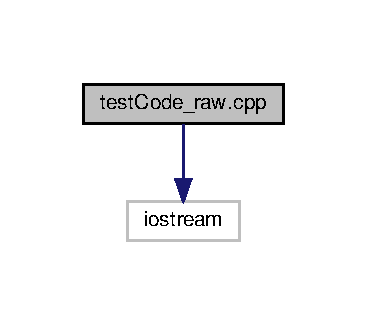
\includegraphics[width=176pt]{testCode__raw_8cpp__incl}
\end{center}
\end{figure}
\subsection*{Functions}
\begin{DoxyCompactItemize}
\item 
void \hyperlink{testCode__raw_8cpp_a6b065b21c39a8398f50a16c10a711deb}{print\+Num} (int num)
\begin{DoxyCompactList}\small\item\em Prints given input number. \end{DoxyCompactList}\item 
int \hyperlink{testCode__raw_8cpp_ab6930ae083d5370c3f09fba32d41e16e}{add\+One} (int num)
\begin{DoxyCompactList}\small\item\em Adds 1 to given input number. \end{DoxyCompactList}\item 
int \hyperlink{testCode__raw_8cpp_ae66f6b31b5ad750f1fe042a706a4e3d4}{main} ()
\end{DoxyCompactItemize}


\subsection{Function Documentation}
\mbox{\Hypertarget{testCode__raw_8cpp_ab6930ae083d5370c3f09fba32d41e16e}\label{testCode__raw_8cpp_ab6930ae083d5370c3f09fba32d41e16e}} 
\index{test\+Code\+\_\+raw.\+cpp@{test\+Code\+\_\+raw.\+cpp}!add\+One@{add\+One}}
\index{add\+One@{add\+One}!test\+Code\+\_\+raw.\+cpp@{test\+Code\+\_\+raw.\+cpp}}
\subsubsection{\texorpdfstring{add\+One()}{addOne()}}
{\footnotesize\ttfamily int add\+One (\begin{DoxyParamCaption}\item[{int}]{num }\end{DoxyParamCaption})}



Adds 1 to given input number. 


\begin{DoxyParams}{Parameters}
{\em num} & input number\\
\hline
\end{DoxyParams}
Just adds 1 to input number \begin{DoxyReturn}{Returns}
num+1 
\end{DoxyReturn}


Definition at line 34 of file test\+Code\+\_\+raw.\+cpp.

\mbox{\Hypertarget{testCode__raw_8cpp_ae66f6b31b5ad750f1fe042a706a4e3d4}\label{testCode__raw_8cpp_ae66f6b31b5ad750f1fe042a706a4e3d4}} 
\index{test\+Code\+\_\+raw.\+cpp@{test\+Code\+\_\+raw.\+cpp}!main@{main}}
\index{main@{main}!test\+Code\+\_\+raw.\+cpp@{test\+Code\+\_\+raw.\+cpp}}
\subsubsection{\texorpdfstring{main()}{main()}}
{\footnotesize\ttfamily int main (\begin{DoxyParamCaption}{ }\end{DoxyParamCaption})}

$<$ Use some random value as input to the code 

Definition at line 38 of file test\+Code\+\_\+raw.\+cpp.

\mbox{\Hypertarget{testCode__raw_8cpp_a6b065b21c39a8398f50a16c10a711deb}\label{testCode__raw_8cpp_a6b065b21c39a8398f50a16c10a711deb}} 
\index{test\+Code\+\_\+raw.\+cpp@{test\+Code\+\_\+raw.\+cpp}!print\+Num@{print\+Num}}
\index{print\+Num@{print\+Num}!test\+Code\+\_\+raw.\+cpp@{test\+Code\+\_\+raw.\+cpp}}
\subsubsection{\texorpdfstring{print\+Num()}{printNum()}}
{\footnotesize\ttfamily void print\+Num (\begin{DoxyParamCaption}\item[{int}]{num }\end{DoxyParamCaption})}



Prints given input number. 


\begin{DoxyParams}{Parameters}
{\em num} & input number\\
\hline
\end{DoxyParams}
Provision to print numbers from single place While using multi-\/threading can be used lock here 

Definition at line 24 of file test\+Code\+\_\+raw.\+cpp.


\hypertarget{testCode__subl_8cpp}{}\section{test\+Code\+\_\+subl.\+cpp File Reference}
\label{testCode__subl_8cpp}\index{test\+Code\+\_\+subl.\+cpp@{test\+Code\+\_\+subl.\+cpp}}
{\ttfamily \#include $<$iostream$>$}\newline
Include dependency graph for test\+Code\+\_\+subl.\+cpp\+:\nopagebreak
\begin{figure}[H]
\begin{center}
\leavevmode
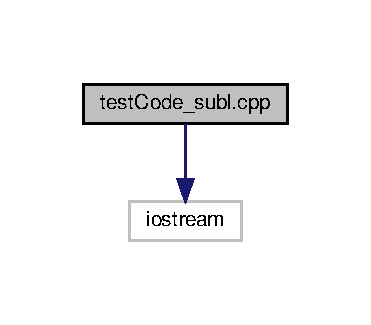
\includegraphics[width=178pt]{testCode__subl_8cpp__incl}
\end{center}
\end{figure}
\subsection*{Functions}
\begin{DoxyCompactItemize}
\item 
void \hyperlink{testCode__subl_8cpp_a6b065b21c39a8398f50a16c10a711deb}{print\+Num} (int num)
\begin{DoxyCompactList}\small\item\em Prints a number. \end{DoxyCompactList}\item 
int \hyperlink{testCode__subl_8cpp_ab6930ae083d5370c3f09fba32d41e16e}{add\+One} (int num)
\begin{DoxyCompactList}\small\item\em Adds one. \end{DoxyCompactList}\item 
int \hyperlink{testCode__subl_8cpp_ae66f6b31b5ad750f1fe042a706a4e3d4}{main} ()
\end{DoxyCompactItemize}


\subsection{Function Documentation}
\mbox{\Hypertarget{testCode__subl_8cpp_ab6930ae083d5370c3f09fba32d41e16e}\label{testCode__subl_8cpp_ab6930ae083d5370c3f09fba32d41e16e}} 
\index{test\+Code\+\_\+subl.\+cpp@{test\+Code\+\_\+subl.\+cpp}!add\+One@{add\+One}}
\index{add\+One@{add\+One}!test\+Code\+\_\+subl.\+cpp@{test\+Code\+\_\+subl.\+cpp}}
\subsubsection{\texorpdfstring{add\+One()}{addOne()}}
{\footnotesize\ttfamily int add\+One (\begin{DoxyParamCaption}\item[{int}]{num }\end{DoxyParamCaption})}



Adds one. 


\begin{DoxyParams}[1]{Parameters}
\mbox{\tt in}  & {\em num} & The number\\
\hline
\end{DoxyParams}
\begin{DoxyReturn}{Returns}
\{ num+1 \} 
\end{DoxyReturn}


Definition at line 36 of file test\+Code\+\_\+subl.\+cpp.

\mbox{\Hypertarget{testCode__subl_8cpp_ae66f6b31b5ad750f1fe042a706a4e3d4}\label{testCode__subl_8cpp_ae66f6b31b5ad750f1fe042a706a4e3d4}} 
\index{test\+Code\+\_\+subl.\+cpp@{test\+Code\+\_\+subl.\+cpp}!main@{main}}
\index{main@{main}!test\+Code\+\_\+subl.\+cpp@{test\+Code\+\_\+subl.\+cpp}}
\subsubsection{\texorpdfstring{main()}{main()}}
{\footnotesize\ttfamily int main (\begin{DoxyParamCaption}{ }\end{DoxyParamCaption})}



Definition at line 41 of file test\+Code\+\_\+subl.\+cpp.

\mbox{\Hypertarget{testCode__subl_8cpp_a6b065b21c39a8398f50a16c10a711deb}\label{testCode__subl_8cpp_a6b065b21c39a8398f50a16c10a711deb}} 
\index{test\+Code\+\_\+subl.\+cpp@{test\+Code\+\_\+subl.\+cpp}!print\+Num@{print\+Num}}
\index{print\+Num@{print\+Num}!test\+Code\+\_\+subl.\+cpp@{test\+Code\+\_\+subl.\+cpp}}
\subsubsection{\texorpdfstring{print\+Num()}{printNum()}}
{\footnotesize\ttfamily void print\+Num (\begin{DoxyParamCaption}\item[{int}]{num }\end{DoxyParamCaption})}



Prints a number. 


\begin{DoxyParams}[1]{Parameters}
\mbox{\tt in}  & {\em num} & input number \\
\hline
\end{DoxyParams}


Definition at line 24 of file test\+Code\+\_\+subl.\+cpp.


\hypertarget{testCode__vim_8cpp}{}\section{test\+Code\+\_\+vim.\+cpp File Reference}
\label{testCode__vim_8cpp}\index{test\+Code\+\_\+vim.\+cpp@{test\+Code\+\_\+vim.\+cpp}}
{\ttfamily \#include $<$iostream$>$}\newline
Include dependency graph for test\+Code\+\_\+vim.\+cpp\+:\nopagebreak
\begin{figure}[H]
\begin{center}
\leavevmode
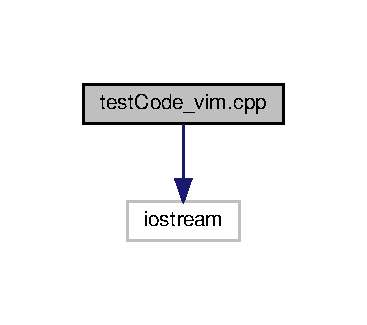
\includegraphics[width=176pt]{testCode__vim_8cpp__incl}
\end{center}
\end{figure}
\subsection*{Functions}
\begin{DoxyCompactItemize}
\item 
void \hyperlink{testCode__vim_8cpp_a6b065b21c39a8398f50a16c10a711deb}{print\+Num} (int num)
\begin{DoxyCompactList}\small\item\em Prints Input Number. \end{DoxyCompactList}\item 
int \hyperlink{testCode__vim_8cpp_ab6930ae083d5370c3f09fba32d41e16e}{add\+One} (int num)
\begin{DoxyCompactList}\small\item\em Adds 1 to input number. \end{DoxyCompactList}\item 
int \hyperlink{testCode__vim_8cpp_ae66f6b31b5ad750f1fe042a706a4e3d4}{main} ()
\end{DoxyCompactItemize}


\subsection{Function Documentation}
\mbox{\Hypertarget{testCode__vim_8cpp_ab6930ae083d5370c3f09fba32d41e16e}\label{testCode__vim_8cpp_ab6930ae083d5370c3f09fba32d41e16e}} 
\index{test\+Code\+\_\+vim.\+cpp@{test\+Code\+\_\+vim.\+cpp}!add\+One@{add\+One}}
\index{add\+One@{add\+One}!test\+Code\+\_\+vim.\+cpp@{test\+Code\+\_\+vim.\+cpp}}
\subsubsection{\texorpdfstring{add\+One()}{addOne()}}
{\footnotesize\ttfamily int add\+One (\begin{DoxyParamCaption}\item[{int}]{num }\end{DoxyParamCaption})}



Adds 1 to input number. 


\begin{DoxyParams}{Parameters}
{\em num} & \\
\hline
\end{DoxyParams}
\begin{DoxyReturn}{Returns}
num+1 
\end{DoxyReturn}


Definition at line 36 of file test\+Code\+\_\+vim.\+cpp.

\mbox{\Hypertarget{testCode__vim_8cpp_ae66f6b31b5ad750f1fe042a706a4e3d4}\label{testCode__vim_8cpp_ae66f6b31b5ad750f1fe042a706a4e3d4}} 
\index{test\+Code\+\_\+vim.\+cpp@{test\+Code\+\_\+vim.\+cpp}!main@{main}}
\index{main@{main}!test\+Code\+\_\+vim.\+cpp@{test\+Code\+\_\+vim.\+cpp}}
\subsubsection{\texorpdfstring{main()}{main()}}
{\footnotesize\ttfamily int main (\begin{DoxyParamCaption}{ }\end{DoxyParamCaption})}



Definition at line 41 of file test\+Code\+\_\+vim.\+cpp.

\mbox{\Hypertarget{testCode__vim_8cpp_a6b065b21c39a8398f50a16c10a711deb}\label{testCode__vim_8cpp_a6b065b21c39a8398f50a16c10a711deb}} 
\index{test\+Code\+\_\+vim.\+cpp@{test\+Code\+\_\+vim.\+cpp}!print\+Num@{print\+Num}}
\index{print\+Num@{print\+Num}!test\+Code\+\_\+vim.\+cpp@{test\+Code\+\_\+vim.\+cpp}}
\subsubsection{\texorpdfstring{print\+Num()}{printNum()}}
{\footnotesize\ttfamily void print\+Num (\begin{DoxyParamCaption}\item[{int}]{num }\end{DoxyParamCaption})}



Prints Input Number. 


\begin{DoxyParams}{Parameters}
{\em num} & \\
\hline
\end{DoxyParams}


Definition at line 24 of file test\+Code\+\_\+vim.\+cpp.


%--- End generated contents ---

% Index
\backmatter
\newpage
\phantomsection
\clearemptydoublepage
\addcontentsline{toc}{chapter}{Index}
\printindex

\end{document}
